\subsection{Slave Switch Module (SS)}
\label{sec:SS}


The Slave Switch Module (SS) controls the power supply to the Slave Module (SL).
As explained previously in section \ref{sec:Too}, the slave is powered only during transmission in order
to reduce energy consumption mainly due to the relatively high standby current of the radio module.

\subsubsection*{Requirements}


The load switch must be able to switch the maximum current for both master and slave.
The maximum current is determined by the GMS module on the slave.
We expect the maximum to not exceed \SI{1}{\A}.

\subsubsection*{Implementation}


\begin{figure}[h]
    \centering
    \includegraphics[width=0.3\textwidth]{MA/SS/SS}
    \caption{SS - schematic, based on datasheet \cite{noauthor_tps22810_2016}}
\end{figure}

\begin{table}[H]
    \centering
    \begin{threeparttable}[b]
        \begin{tabularx}{\linewidth}{ >
                    {\hsize=.25\hsize}X >
                    {\hsize=0.5\hsize}X >
                    {\hsize=.25\hsize}X  >
                    {\hsize=.5\hsize}X >
                    {\hsize=.25\hsize}X  >
                    {\hsize=3\hsize}X
            }
                  & \multicolumn{4}{c}{Pin mapping} &                                                                   \\
            \cmidrule(lr){3-6}
            Id    & Net                             & Nb. & Name             & Type            & Function               \\
            \midrule
            $U_1$ & .5V                             & 1   & VIN              & \leftharpoonup  & input                  \\
            $U_1$ & \Gnd                            & 2   & \texttt{GND}     & \Gnd            &                        \\
            $U_1$ & .ESL                            & 3   & \texttt{EN/UVLO} & \rightharpoonup & switch enable          \\
            $U_1$ &                                 & 4   & \texttt{CT}      &                 & left floating\tnote{1} \\
            $U_1$ &                                 & 5   & \texttt{QOD}     &                 & left floating\tnote{2} \\
            $U_1$ & .V\textsubscript{\mu S}         & 6   & \texttt{VOUT}    & \rightharpoonup & output                 \\
        \end{tabularx}
        \begin{tablenotes}
            \item [1]  the Arduino is not a high current load for this switch.
            \item [2] we don't care how fast the charge at the output decreases.
        \end{tablenotes}
    \end{threeparttable}

\end{table}
\input{hardware/modules/MA/SS/SS_issues}
\begin{table}[H]
    \centering
    \begin{threeparttable}[b]
        \begin{tabularx}{\linewidth}{ >
                    {\hsize=0.25\hsize}X >
                    {\hsize=0.75\hsize}X >
                    {\hsize=1.25\hsize}X >
                    {\hsize=0.5\hsize}X >
                    {\hsize=2.25\hsize}X
            }
            Id    & BOM Item                      & Order Code       & FF       & Rationale                                                                               \\
            \midrule
            $U_1$ & \cite{noauthor_tps22810_2016} & TPS22810DBVR/710 & SOT-23/6 & low $R_{ON}$\tnote{1}, input voltage range down to \SI{2.7}{\V}, low quiescent current. \\
        \end{tabularx}
        \begin{tablenotes}
            \item [1] The \cite{noauthor_arduino_2016-1} requires a \SI{5}{\V} power supply which is
            regulated to \SI{3.3}{\V} on the board.

            The Arduino board uses the \cite{noauthor_ap7115_2017} voltage regulator.
            According to the datasheet, the dropout voltage is
            \SI{200}{\mV}. Therefore, the voltage supplied to the Arduino $V_{\mu M}$ must be greater than \SI{3.5}{\V}.
        \end{tablenotes}
    \end{threeparttable}
    \caption{SS - BOM}
\end{table}










